\chapter{Аналитическая часть}

\section{Описание предметной области}\label{sec:предмет}

Предметной областью является фитнес-индустрия. Типовой фитнес-клуб предлагает разные фитнес-активности, тренировки и услуги, направленные на улучшение физической формы, приведение в тонус тела и поддержание обего физического и психического благополучия.

Чаще всего в фитнес-клубе есть тренера, клиенты и администраторы.
\begin{enumerate}[label=\arabic*)]
	\item \textbf{Клиент} --- человек, который ходит в фитнес-центр для получения услуг.
	\item \textbf{Тренер} --- это сотрудник фитнес-центра, который проводит тренировки для клиентов.
	\item \textbf{Администратор} --- это сотрудник фитнес-центра, ответственный за управление расписанием фитнес-центра, а также решающий все вопросы клиентов и тренеров.
\end{enumerate}

\section{Анализ существующих решений}

В эпоху цифровых технологий автоматизация процессов имеет огромное значение. Традиционные методы записи на тренировки через звонки или сообщения тренерам часто неудобны и не отвечают потребностям современных клиентов. Поэтому разработка решений, позволяющих клиентам записываться на тренировки онлайн, имеет большое значение.
А так же одной из целей создания фитнес-клуба является мотивирование людей заниматься спортом, так как в России только 4\% населения регулярно занимаются в фитнес-клубах, что в 3 раза меньше, чем в Европе~\cite{stat1}.

На данный момент в России существует множество фитнес-клубов. Я рассмотрю самые популярные из них, а именно XFit~\cite{xfit}, WeGym~\cite{wegym} и фитнес-клуб СССР~\cite{sssr}.

Существующие решения анализировались по следующим критериям:
\begin{enumerate}[label=\arabic*)]
	\item возможность просмотра расписания с фильтрацией;
	\item наличие онлайн-записи на тренировки;
	\item разнообразие групповых занятий (более 3 видов тренировок);
	\item возможность просмотра информации о тренерах;
	\item наличие бонусной системы.
\end{enumerate}

\begin{table}[h]
	\begin{center}
		\begin{threeparttable}
			\captionsetup{justification=raggedright,singlelinecheck=off}
			\caption{\label{tbl:solve} Анализ существующих решений}
			\begin{tabular}{|p{6cm}|p{3cm}|p{3cm}|p{3cm}|}
				\hline  & XFit & WeGym  & СССР \\ \hline
				Расписание с фильтрацией & + & + & -  \\ \hline
				Разнообразие групповых занятий & + & + & -  \\ \hline
				Онлайн-запись на тренировки & -  & - & - \\ \hline
				Возможность просмотра информации о тренерах & + & + & + \\ \hline
				Наличие бонусной системы & + & - & - \\ \hline
			\end{tabular}
		\end{threeparttable}
	\end{center}
\end{table}

\section{Формализация задачи}\label{sec:формализация}

В ходе выполнения курсовой работы необходимо спроектировать и разработать базу данных для хранения и обработки данных фитнес-клуба, а так же веб-приложение для взаимодействия с ним.
На основании анализа предметной области в фитнес-клубе могут быть выделены следующие роли.
\begin{enumerate}[label=\arabic*)]
	\item Гость --- это посетитель фитнес-центра, который еще не зарегистрировался на сайте или не вошел в свою учетную запись. Он не имеет доступа к личным данным, функциям бонусной программы, онлайн-записи на тренировки или другим привилегиям, доступным только зарегистрированным пользователям.
	\item Клиент --- это зарегистрированный пользователь фитнес-центра, который имеет доступ к своей учетной записи. Он может просматривать расписание занятий, записываться на тренировки, участвовать в бонусной программе, получать информацию о тренировках, услугах и специальных предложениях.
	\item Тренер --- это сотрудник фитнес-центра, который проводит тренировки для клиентов. Тренер может оформлять свои персональные тренировки в расписании и просматривать информацию о клиентах.
	\item Администратор --- это сотрудник фитнес-центра, ответственный за управление сайтом и контентом. Он имеет доступ к административным функциям, таким как создание и редактирование расписания тренировок, управление информацией о тренерах, настройка бонусной программы, управление акциями и специальными предложениями, а также учетом клиентов и их данных.
\end{enumerate}

На рисунках \ref{fig:usecase_guest}--\ref{fig:usecase_admin} изображены диаграммы вариантов использования для разных типов пользователей.

\begin{figure}[h!]
	\centering
	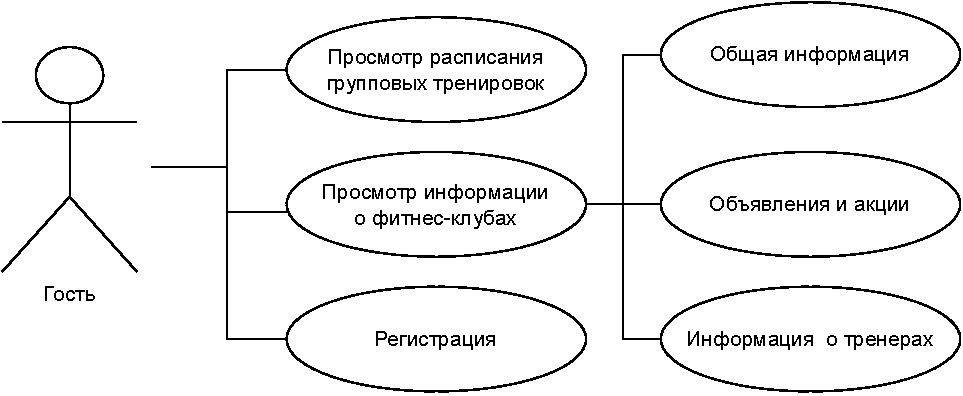
\includegraphics[width=0.7\linewidth]{img/usecase-guest}
	\caption{Диаграмма вариантов использования для гостя}
	\label{fig:usecase_guest}
\end{figure}

\begin{figure}[h!]
	\centering
	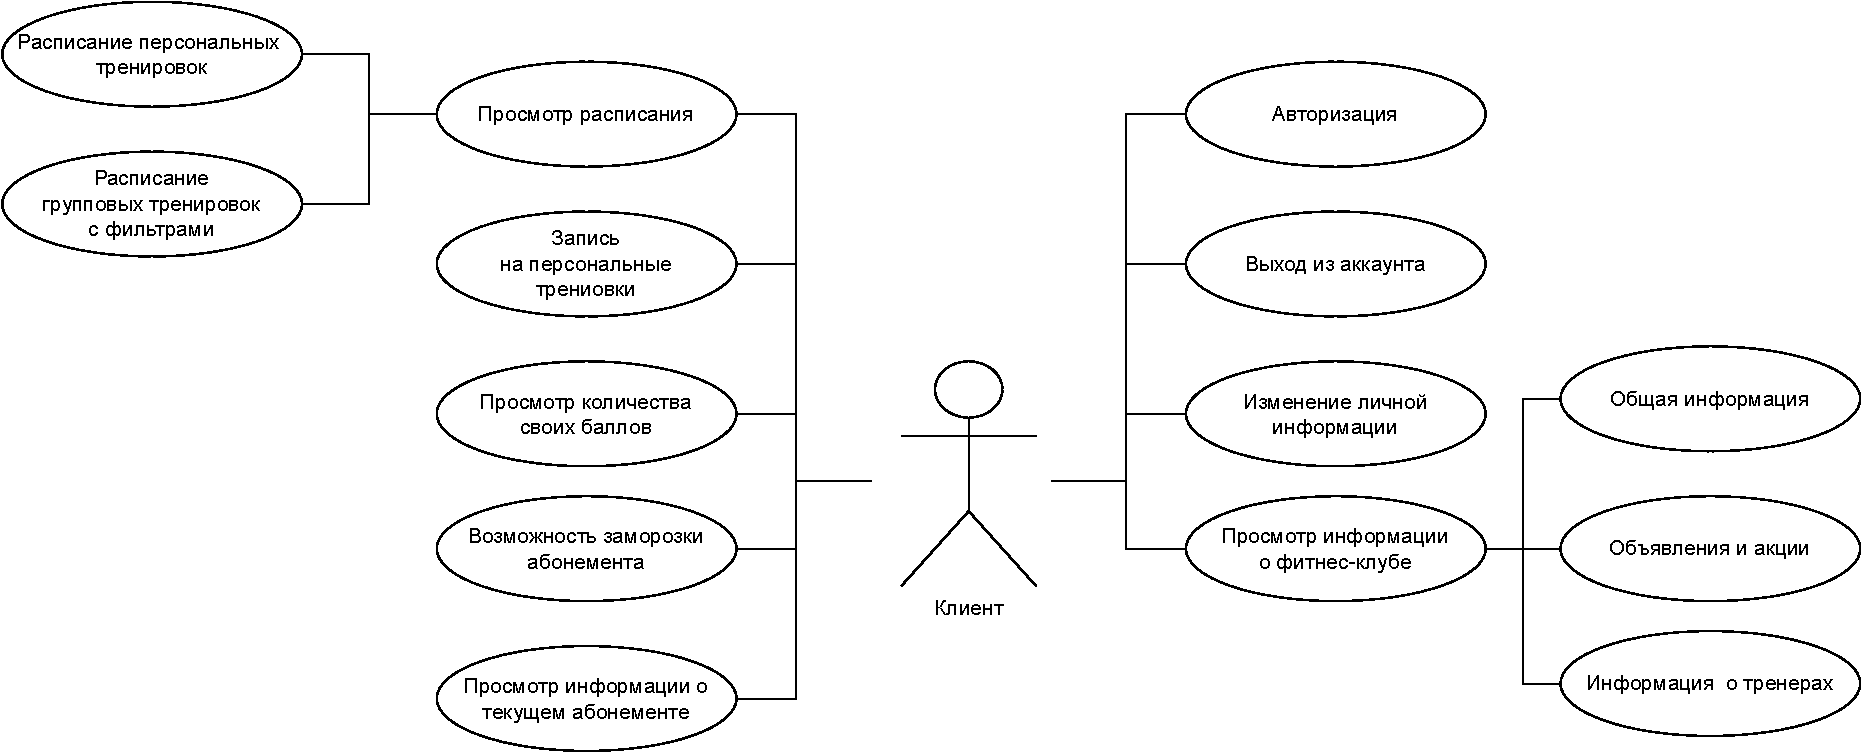
\includegraphics[width=0.95\linewidth]{img/usecase-client}
	\caption{Диаграмма вариантов использования диаграмма для клиента}
	\label{fig:usecase_client}
\end{figure}
\clearpage

\begin{figure}[h!]
	\centering
	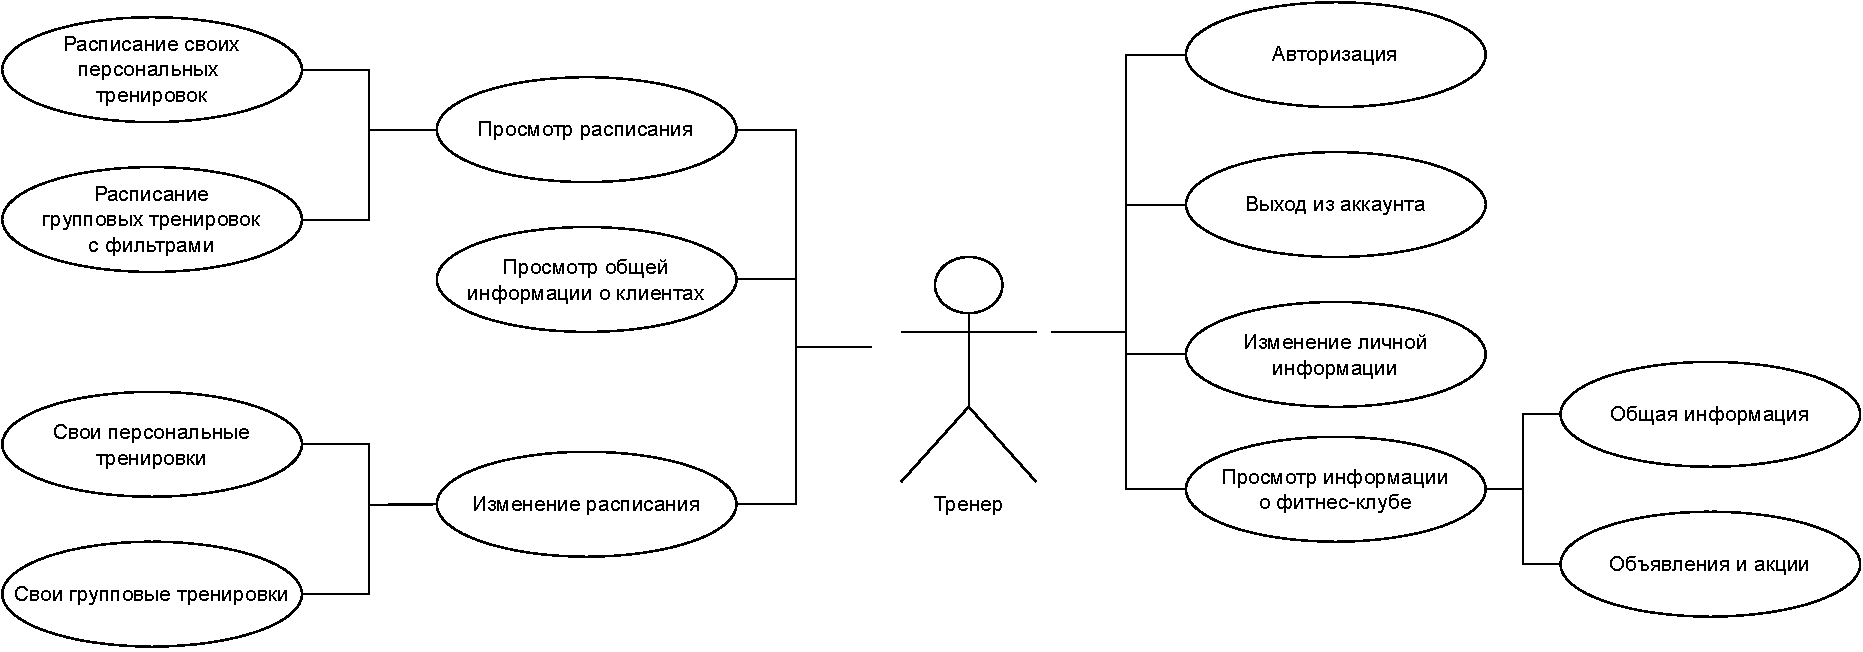
\includegraphics[width=0.95\linewidth]{img/usecase-trainer}
	\caption{Диаграмма вариантов использования диаграмма для тренера}
	\label{fig:usecase_trainer}
\end{figure}

\begin{figure}[h!]
	\centering
	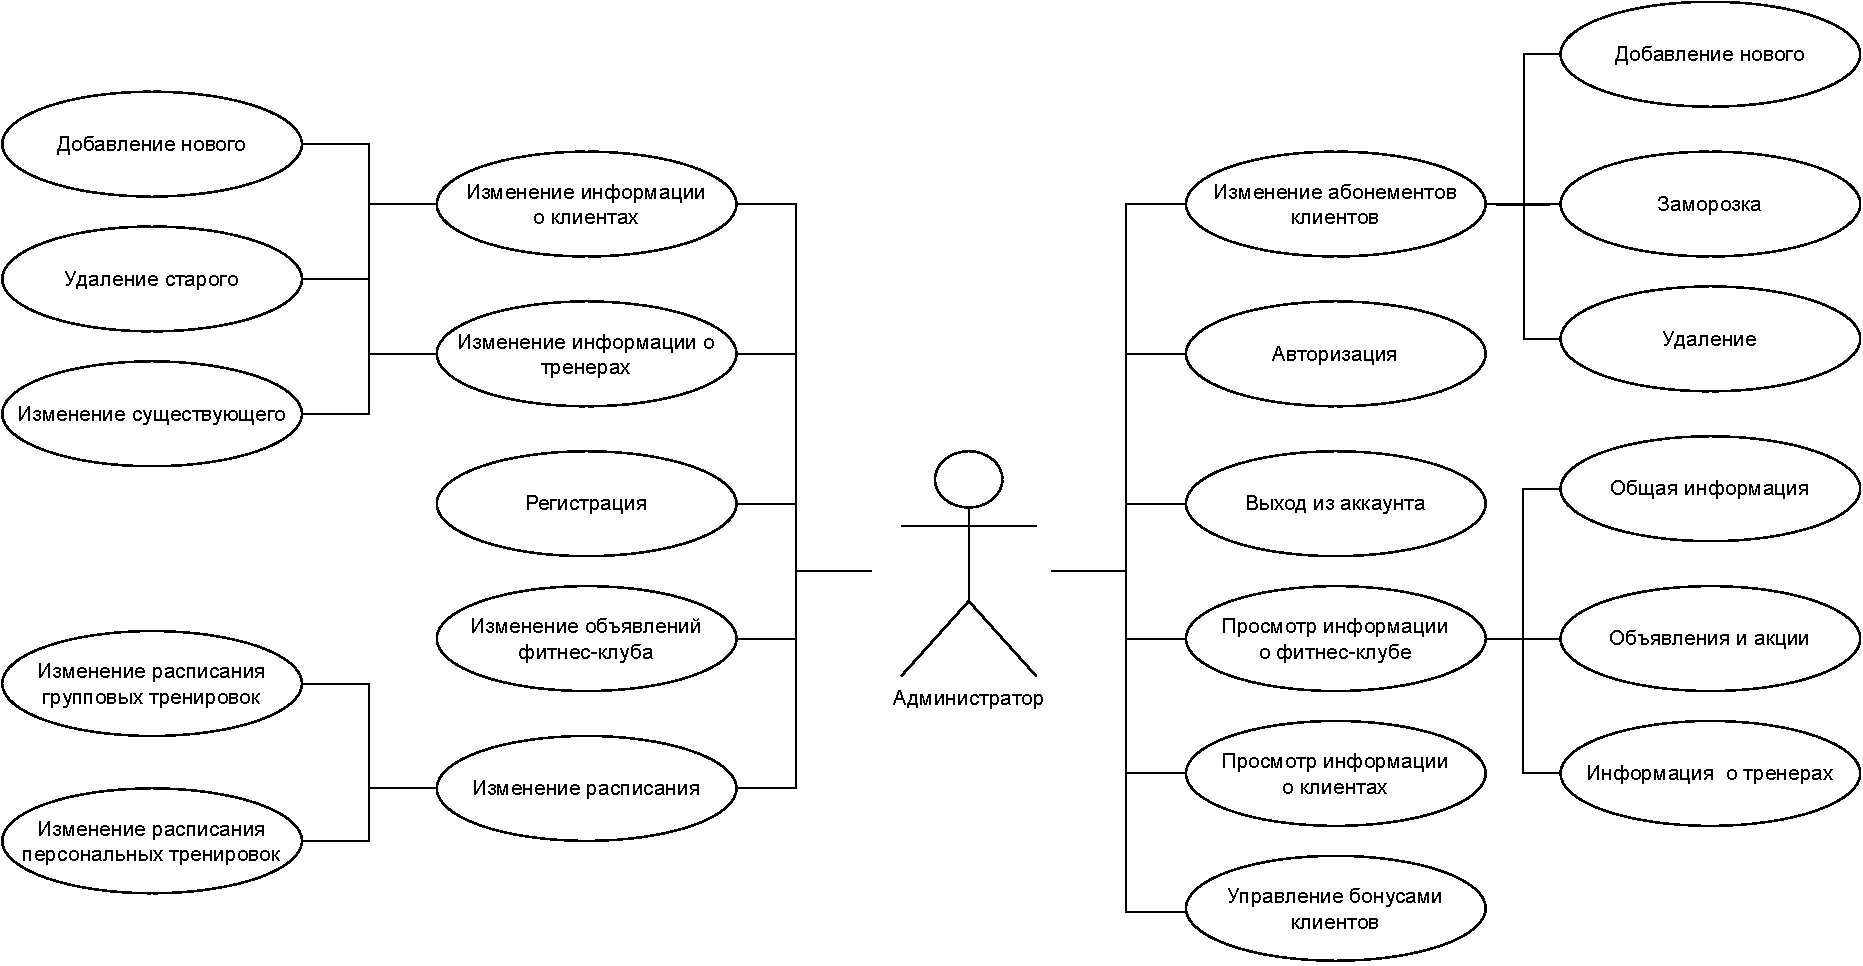
\includegraphics[width=\linewidth]{img/usecase-admin}
	\caption{Диаграмма вариантов использования диаграмма для администратора}
	\label{fig:usecase_admin}
\end{figure}


Для создания базы данных фитнес-центра, были выделены следующие сущности:
\begin{enumerate}[label=\arabic*)]
	\item пользователи;
	\item администраторы;
	\item клиенты;
	\item тренера;
	\item расписание;
	\item абонементы;
	\item бонусы;
	\item тренировки;
	\item услуги и товары.
\end{enumerate}

ER-диаграмма сущностей в нотации Чена представлена на рисунке~\ref{fig:er}.
\clearpage

\begin{figure}[h!]
	\centering
	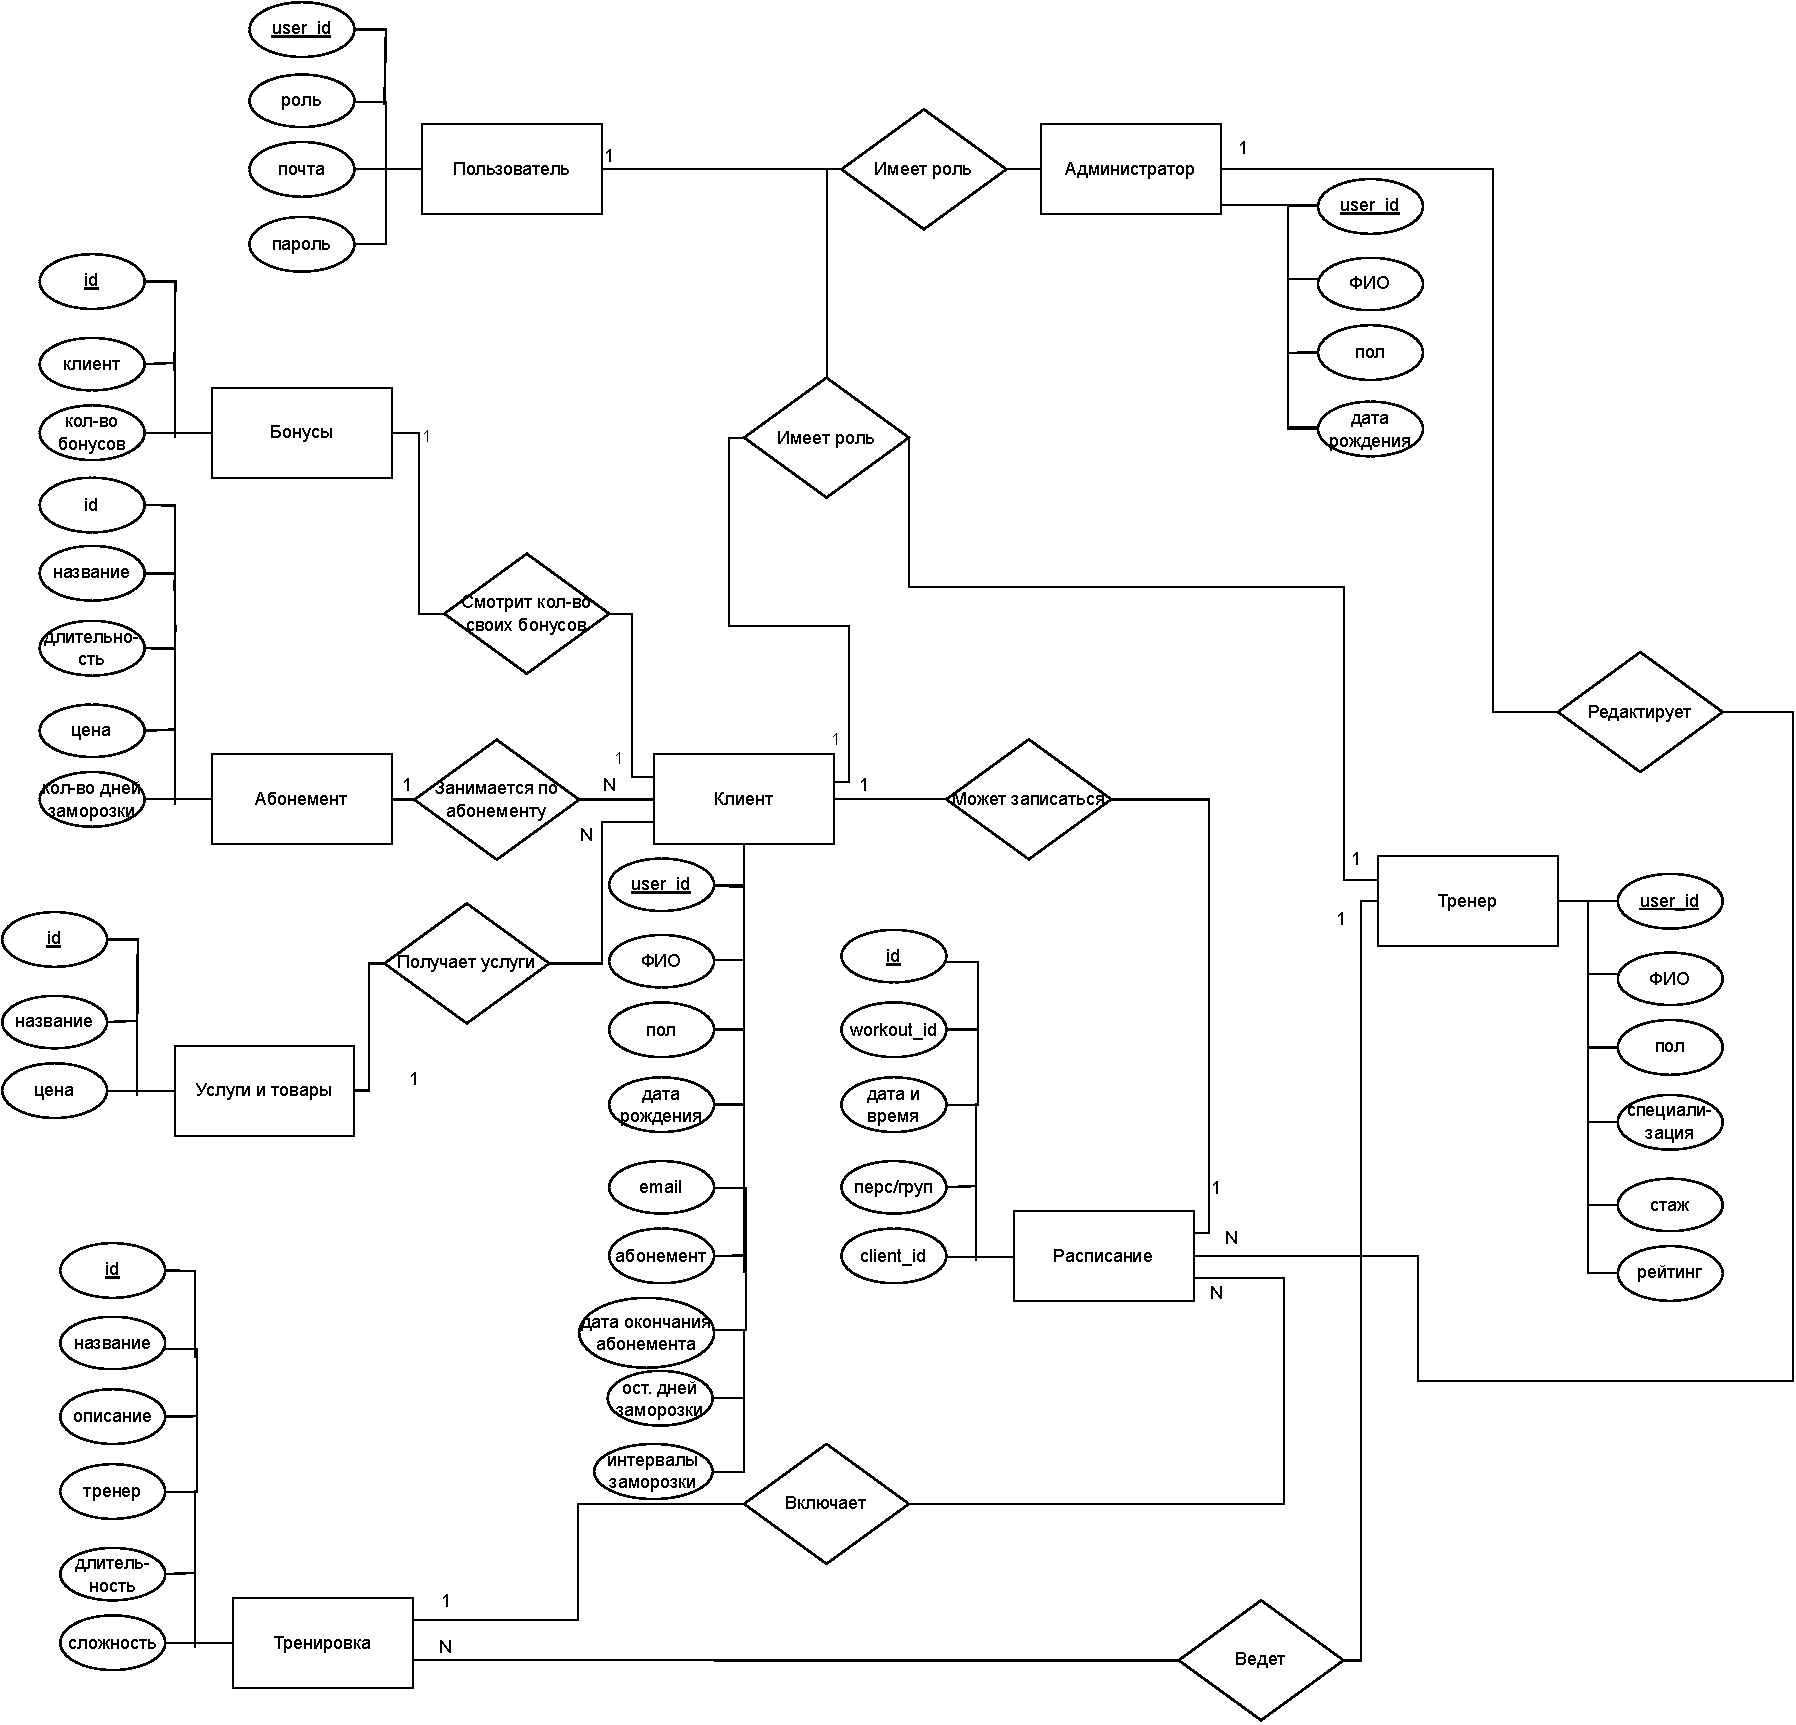
\includegraphics[width=\linewidth]{img/er}
	\caption{ER-диаграмма сущностей в нотации Чена}
	\label{fig:er}
\end{figure}


\section{Виды баз данных}

База данных представляет собой совокупность специальным образом организованных данных, хранимых в памяти вычислительной системы и отображающих состояние объектов и их взаимосвязей в рассматриваемой предметной области. Она играет важную роль в хранении, управлении, анализе и обработке данных, что в конечном итоге облегчает принятие решений и повышает эффективность работы организаций и систем~\cite{serg}.

По типу модели данных базы данных разделяются на следующие~\cite{ucheb}:
\begin{enumerate}[label=\arabic*)]
	\item дореляционные;
	\item реляционные;
	\item постреляционные.
\end{enumerate}

\subsection{Дореляционные базы данных}

Дореляционные базы данных --- это тип баз данных, который находится за пределами реляционной модели. Они предоставляют альтернативные способы организации и хранения данных, не используя таблицы, столбцы и отношения, как это делается в реляционных базах данных.

Дореляционные базы данных можно разделить на 3 категории~\cite{deit}:
\begin{enumerate}[label=\arabic*)]
	\item с инвертированными списками;
	\item иерархические;
	\item сетевые.
\end{enumerate}

В дореляционных базах данных на основе инвертированных списков каждый уникальный атрибут собирается в отдельный список, содержащий ссылки на элементы данных с соответствующим значением. Это позволяет гибко и эффективно осуществлять поиск, фильтрацию и полнотекстовый поиск данных. 
В иерархических базах данных данные огранизованы в иерархическую структуру подобно древовидной структуре. В такой базе данных каждый элемент данных имеет связь с одним родительским элементом и может иметь несколько дочерних элементов.
В сетевых база данных информация организована в виде графа. В таких базах данных сущности представлены в виде вершин, а связи между сущностями --- в виде ребер графа~\cite{gavr}.

\subsection{Реляционные базы данных}

Реляционные базы данных основаны на реляционной модели, которая представляет данные в виде таблиц с записями и атрибутами. Каждая запись имеет уникальный идентификатор (ключ), а каждый атрибут содержит значение для каждой записи~\cite{rel2}.

Реляционные базы данных отделяют логические структуры данных, такие как таблицы, представления и индексы, от физических структур хранения данных. Это означает, что администраторы баз данных могут управлять физическим хранилищем данных независимо от доступа к данным~\cite{rel}. 

Четыре важные свойства реляционной базы данных определяют ACID~\cite{rel}.
\begin{enumerate}[label=\arabic*)]
	\item Атомарность: все операции в базе данных либо выполняются полностью, либо не выполняются вообще.
	\item Согласованность: после завершения транзакции данные остаются в цельном, согласованном состоянии.
	\item Изоляция: эффекты одной транзакции невидимы для других, пока она не завершится, чтобы избежать несогласованности данных.
	\item Долговечность: реляционная база данных гарантирует, что изменения данных, подтвержденные транзакцией, сохранятся постоянно.
\end{enumerate}

\subsection{Постреляционные базы данных}

Постреляционные базы данных представляют собой различные модели данных, которые расширяют и дополняют возможности классической реляционной модели~\cite{post}. 
Некоторые из основных типов постреляционных моделей представлены далее~\cite{ucheb}.
\begin{enumerate}[label=\arabic*)]
	\item Объектно-реляционные базы данных: они комбинируют функциональность реляционных баз данных с возможностями объектно-ориентирован-ного программирования, что позволяет хранить и обрабатывать сложные объекты со связями и наследованием, предоставляя расширенную модель данных.
	\item Объектно-ориентированные базы данных: они предназначены для хранения объектов и связей между ними без использования традиционных таблиц и отношений. Это позволяет более натурально моделировать и обрабатывать данные, основываясь на концепциях классов, объектов и наследования.
	\item Многомерные базы данных: они предназначены для хранения и обработки многомерных данных, таких как данные OLAP (Online Analytical Processing). Многомерные базы данных оптимизированы для аналитических задач, где данные организованы по нескольким измерениям и иерархиям, что облегчает анализ и отчетность.
	\item Прочие (NoSQL) базы данных: это семейство баз данных, которые не следуют традиционной реляционной модели и предлагают альтернативные подходы к хранению и обработке данных. 
\end{enumerate}

Одним из преимуществ постреляционной модели является возможность объединения связанных реляционных таблиц в одну постреляционную таблицу. Однако, недостатком такой модели является сложность обеспечения целостности и согласованности данных, что может представлять проблемы при работе с ней~\cite{post}.

\clearpage
\section*{Выводы к аналитической части}

В этой части работы был проведен анализ существующих решений и формализованна задача.
Также выбрана реляционная модель данных, так как она подходит для решения поставленной задачи.

\begin{table}[h]
	\begin{center}
		\begin{threeparttable}
			\captionsetup{justification=raggedright,singlelinecheck=off}
			\caption{\label{tbl:bds} Сравнение баз данных}
			\begin{tabular}{|p{3.5cm}|p{3.5cm}|p{3.5cm}|p{3.8cm}|}
				\hline
				& Дореляционные БД & Реляционные БД & Постреляционные БД \\
				\hline
				Организация данных & Иерархическая или сетевая структура & Таблицы, столбцы, отношения & Модели данных, такие как объекты, документы, графы и др. \\
				\hline
				Поддерживаемые типы данных & Ограниченные & Все основные, которые может включать база данных & Расширенные, включая мультимедийные \\
				\hline
				Поддержка транзакционности & нет & есть & есть \\
				\hline
				Опыт работы исполнителя & нет & есть & нет \\
				\hline
			\end{tabular}
		\end{threeparttable}
\end{center}
\end{table}